\documentclass[/home/jesse/Analysis/FemtoAnalysis/AnalysisNotes/AnalysisNoteJBuxton.tex]{subfiles}
\begin{document}

\subsection{$\Xi$ Reconstruction}
\label{CascadeReconstruction}

Our motivation for studying \XiKpm systems is to attempt to better understand the striking difference in the \LamKchP and \LamKchM data at low \kstar (Figure \ref{fig:cLamcKchCfs0010}).

The reconstruction of $\Xi$ particles is one level above V0 reconstruction.  V0 particles are topologically reconstructed by searching for the charged daughters' tracks into which they decay.  With $\Xi$ particles, we search for the V0 particle and charged daughter into which the $\Xi$ decays.  In the case of $\Xi^{-}$, we search for the \Lam (V0) and $\pi^{-}$ (track) daughters.  We will refer to this $\pi$ as the ``bachelor $\pi$".

The following cuts were used to select good $\Xi^{-}$ ($\bar{\Xi}^{+}$) candidates:

\begin{enumerate} 
 \item Shared Daughter Cut for $\Xi$ Collection
 \begin{itemize}
  \item Iterate through $\Xi$ collection to ensure that no daughter is used in more than one $\Xi$ candidate
  \item Remove any candidate in which the bachelor $\pi$ is also a daughter of the \Lam (implemented in AliFemtoXiTrackPairCut class)
 \end{itemize} 
 
\end{enumerate}


\begin{table}[htbp]
 \centering 
%  \renewcommand{\arraystretch}{1.5}
  \begin{tabular}{lc|c|l}
   \hline  
   \multicolumn{4}{c}{\textbf{$\Xi$ reconstruction}} \\
   \hline
   \multicolumn{3}{l|}{$|\eta|$} & $< 0.8$ \\
   \hline
   \multicolumn{3}{l|}{$p_{\mathrm{T}}$} & $> 0.8$ GeV/\textit{c} \\
   \hline
   \multicolumn{3}{l|}{$|m_{\mathrm{inv}} - m_{\mathrm{PDG}}|$} & $< 3.0$ MeV \\ 
   \hline
   \multicolumn{3}{l|}{DCA to prim. vertex} & $<$ 0.3 cm \\
   \hline
   \multicolumn{3}{l|}{Cosine of pointing angle} & $>$ 0.9992 \\
   \hline
   
   \multicolumn{4}{c}{\textbf{\Lam daughter cuts}} \\
   \hline
   \multicolumn{3}{l|}{DCA to prim. vertex} & $>$ 0.2 cm \\
   \hline
   \multicolumn{3}{l|}{Cosine of pointing angle} & $>$ 0.0 \\
   \hline
   \multicolumn{3}{l|}{Cosine of pointing angle to $\Xi$ decay vertex} & $>$ 0.9993 \\
   \hline
   \multicolumn{3}{l|}{OnFlyStatus} & false \\
   \hline
   \multicolumn{4}{l}{All other \Lam and corresponding ($\pi$ and p) daughter cuts are} \\ 
   \multicolumn{4}{l}{same as in primary \Lam selection, and can be found in Sec. \ref{LambdaReconstruction}} \\
   \hline
   
   \multicolumn{4}{c}{\textbf{Bachelor $\boldsymbol\pi$ cuts}} \\
   \hline
   \multicolumn{3}{l|}{$|\eta|$} &  $< 0.8$ \\
   \hline
   \multicolumn{3}{l|}{$p_{\mathrm{T}}$} & $> 0.0$ GeV/\textit{c} \\
   \hline
   \multicolumn{3}{l|}{DCA to prim. vertex} & $>$ 0.1 cm \\
   \hline
   \multicolumn{3}{l|}{Number of clusters in the TPC} & $>$ 70 \\
   \hline
   \multicolumn{3}{l|}{Daughter status} & kTPCrefit \\
   \hline
   \multicolumn{4}{l}{TPC and TOF N$\sigma$ Cuts} \\
   \hline
    & \multicolumn{1}{c}{$p <$ 0.5 GeV/\textit{c}} &  & N$\sigma_{\mathrm{TPC}} <$ 3 \\
   \hline
    & \multirow{2}{*}{$p >$ 0.5 GeV/\textit{c}} &  if TOF \& TPC available & N$\sigma_{\mathrm{TPC}} <$ 3 \& N$\sigma_{\mathrm{TOF}} <$ 3 \\
   \cline{3-4}
    & & else & N$\sigma_{\mathrm{TOF}} <$ 3 \\
   \hline
  \end{tabular}
% \end{minipage}
 \caption[$\Xi$ reconstruction]{$\Xi$ reconstruction}
 \label{tab:XiCuts} 
\end{table}





\begin{figure}[h!]
  \centering
  %%----start of first subfigure---  
  \subfloat[$\Xi^{-}$ reconstruction.]{
    \label{fig:XiReconstruction:a}
    \includegraphics[width=0.49\textwidth]{3_DataSelection/Figures/XiReconstruction.pdf}}
  %%----start of second subfigure---
  \subfloat[$\Xi^{-}$ daughter reconstruction.]{
    \label{fig:XiReconstruction:b}
    \includegraphics[width=0.49\textwidth]{3_DataSelection/Figures/XiReconstruction_V0Cuts.pdf}}
  %%----overall caption----
  \caption[$\Xi$ Reconstruction]{(Left) $\Xi^{-}$ reconstruction (DCA to primary vertex for $\Xi^{-}$ not shown).  (Right) $\Xi^{-}$ daughter reconstruction.}
  \label{fig:XiReconstruction}
\end{figure}





The purity of our $\Xi$ and $\bar{\Xi}$ collections are calculated just as those of our V0 collections \ref{V0Selection}.
Figure \ref{fig:XiPurity}, which is used to calculate the purity, shows the \minv distribution of our $\Xi$($\bar{\Xi}$) candidates just before the final \minv cut.  Currently, we have Purity($\Xi^{-}$) $\approx$ 90\% and Purity($\bar{\Xi}^{+}$) $\approx$ 92\%.

\begin{figure}[h!]
  \centering
  %%----start of first subfigure---  
  \subfloat[$\Xi^{-}$ Purity]{
    \label{fig:XiPurity:a}
    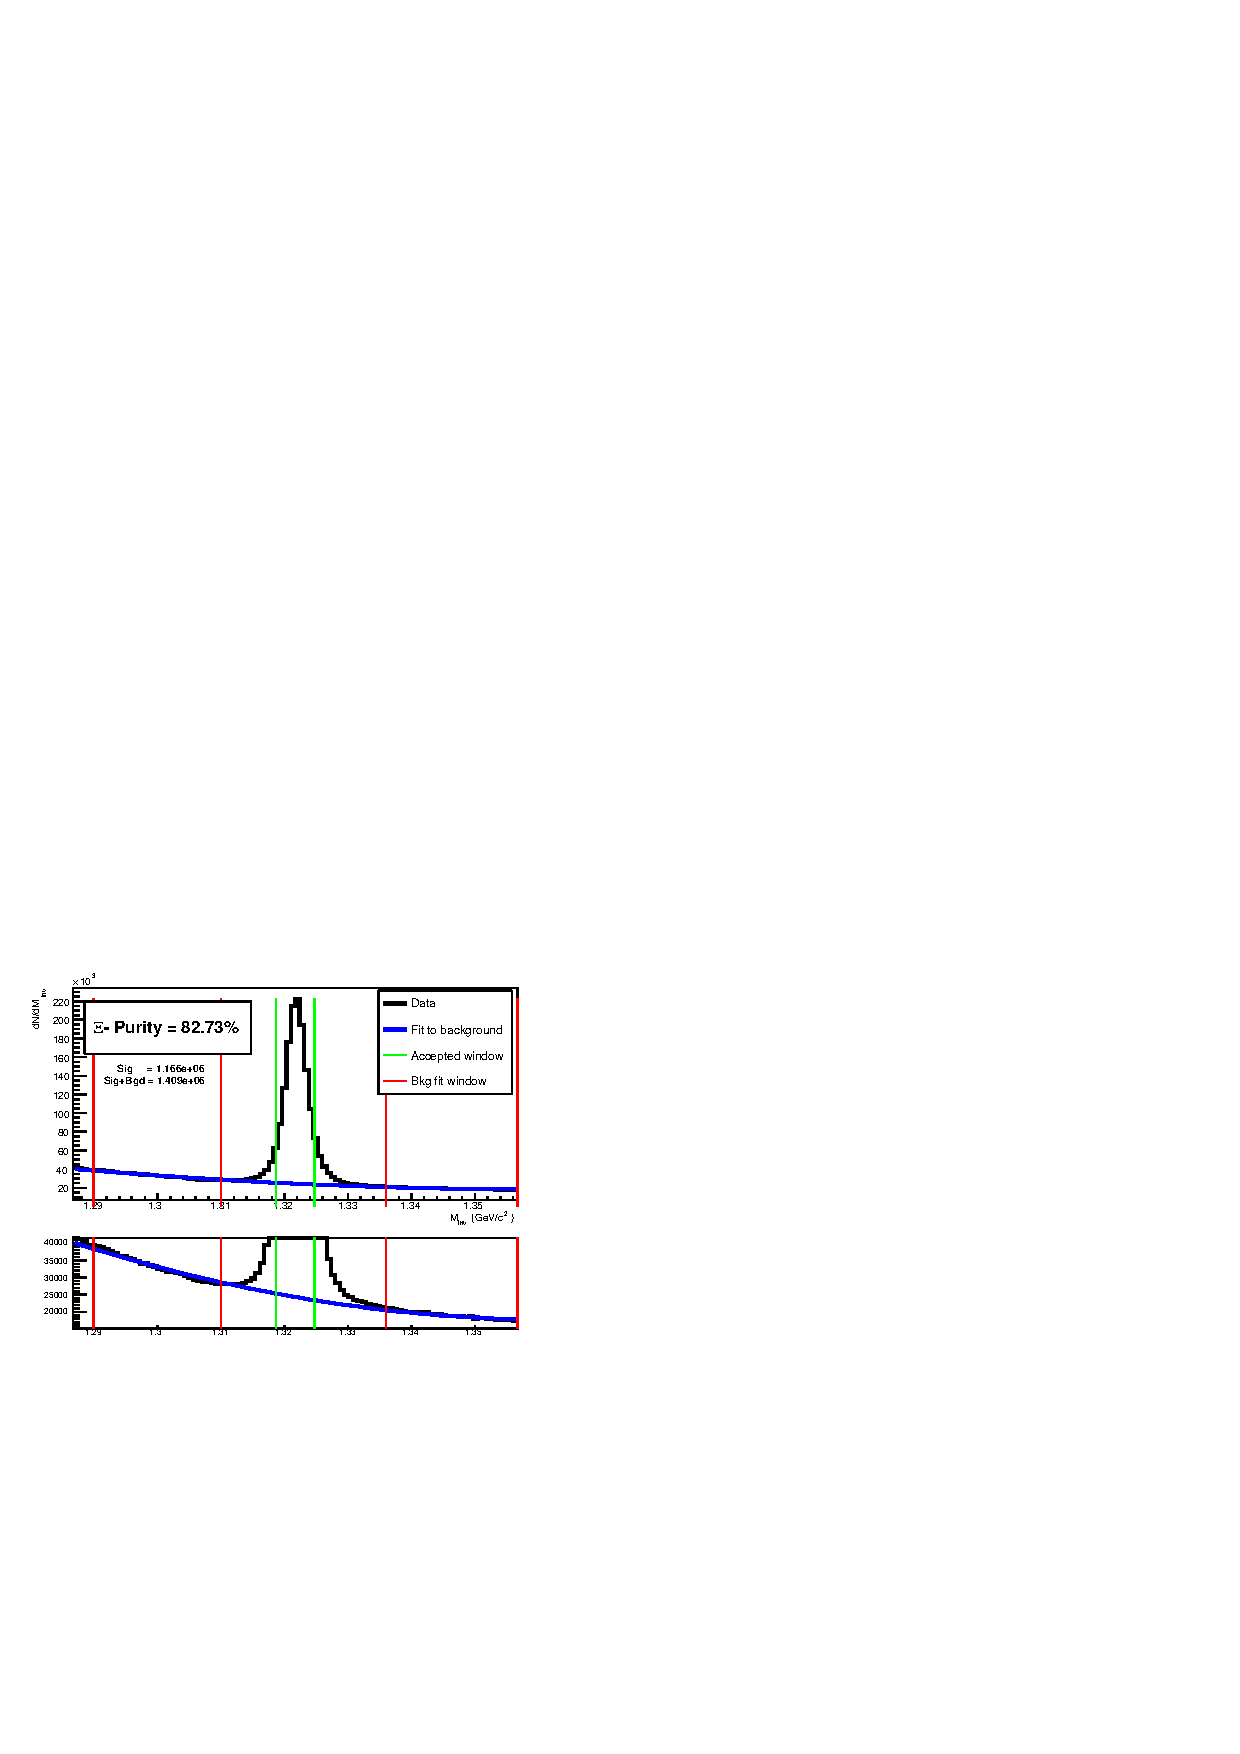
\includegraphics[width=0.49\textwidth]{3_DataSelection/Figures/XiPurity_XiKchP.pdf}}
  %%----start of second subfigure---
  \subfloat[$\bar{\Xi}$ Purity]{
    \label{fig:XiPurity:b}
    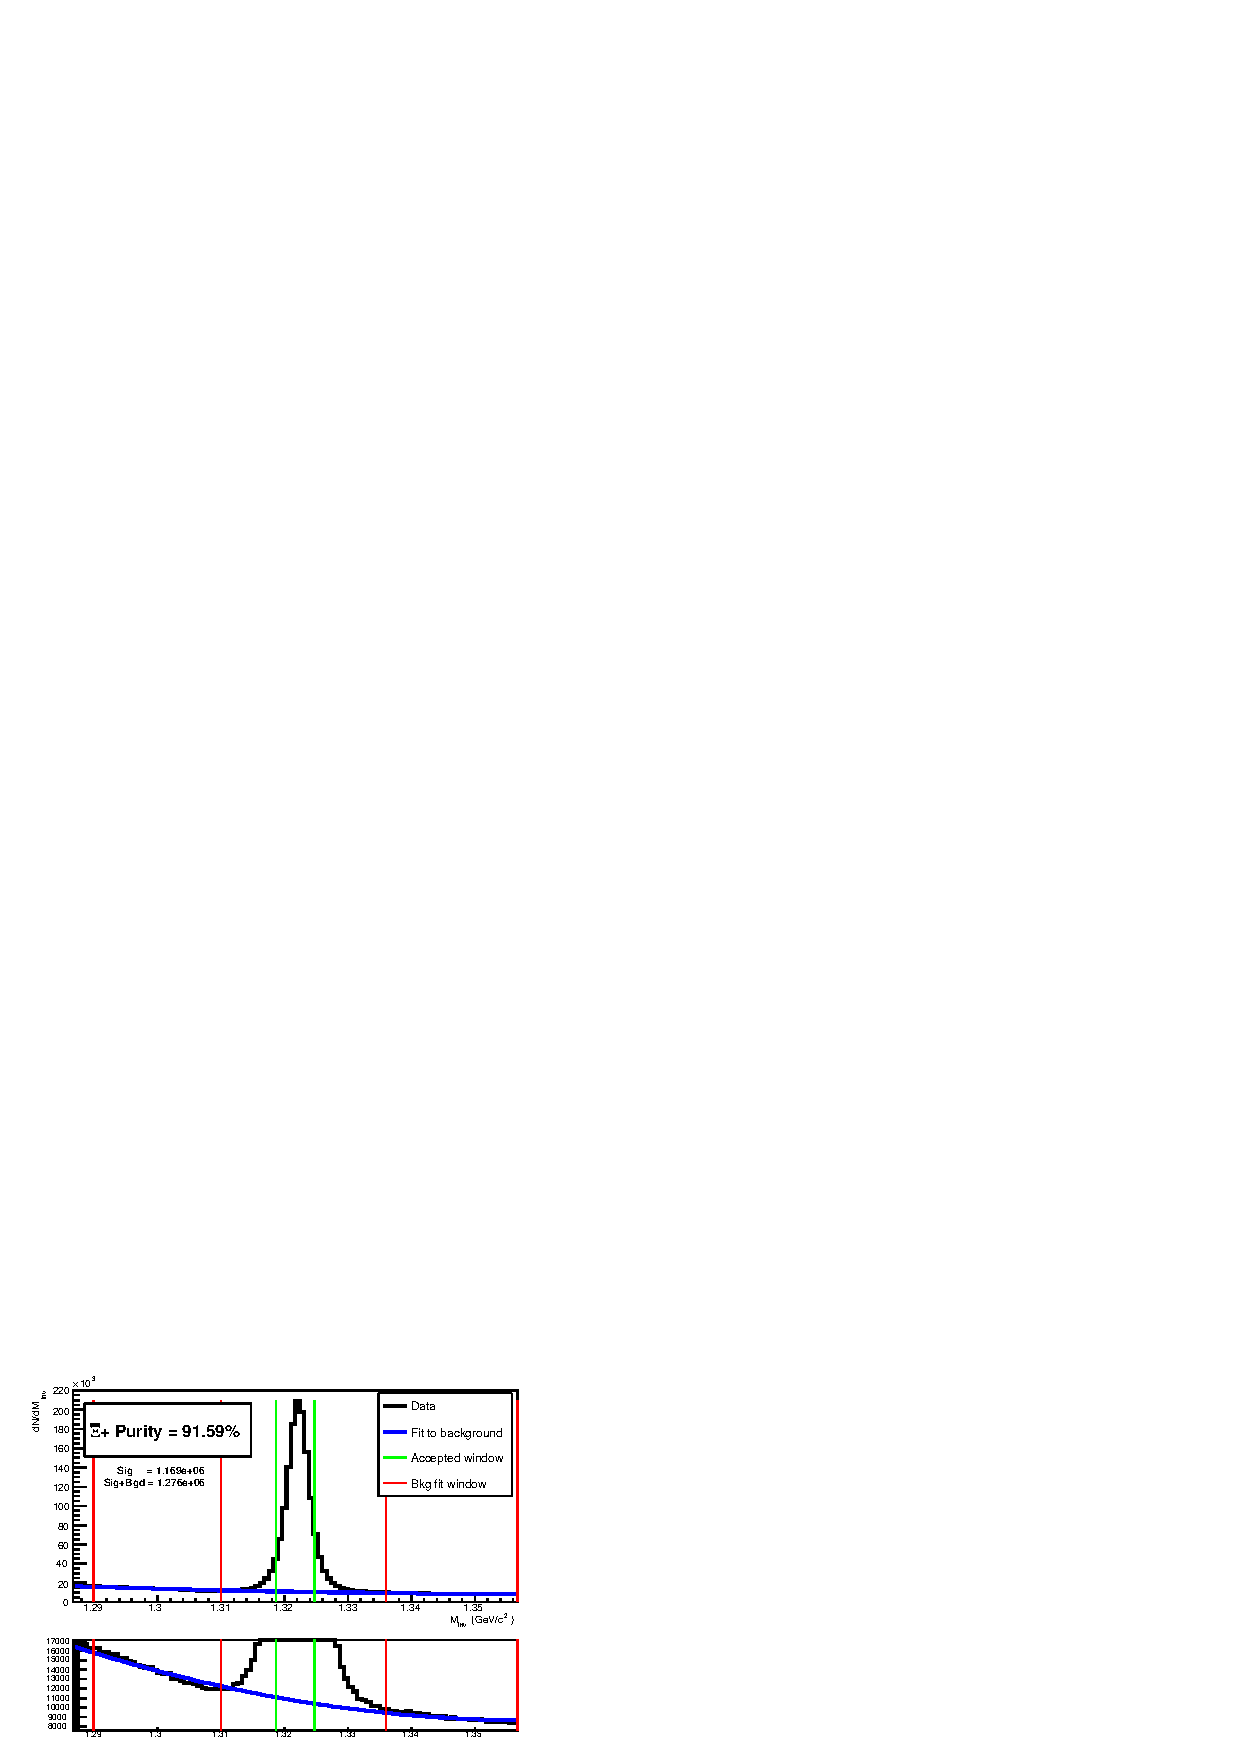
\includegraphics[width=0.49\textwidth]{3_DataSelection/Figures/AXiPurity_AXiKchP.pdf}}
  %%----overall caption----
  \caption[$\Xi^{-}$($\bar{\Xi}^{+}$) Purity]{Invariant mass (\minv) distribution for all $\Xi^{-}$ (a) and $\bar{\Xi}^{+}$ (b) candidates immediately before the final invariant mass cut.  The bottom figures are zoomed to show the background with fit.  The vertical green lines represent the \minv cuts used in the analyses, the red vertical lines delineate the regions over which the background was fit, and the blue line shows the background fit.  These distributions are used to calculate the collection purities, Purity($\Xi^{-}$) $\approx$ 90\% and Purity($\bar{\Xi}^{+}$) $\approx$ 92\%.}
  \label{fig:XiPurity}
\end{figure}

\end{document}